Porphyrine sind organisch-chemische Farbstoffe, die aus 4 Pyrrol-Ringen (Tetrapyrrol) bestehen, die durch vier Methingruppen zyklisch miteinander verbunden sind. Beispiele für Porphyrine sind das Chlorophyll (Farbstoff in Pflanzen) und das Häm in den Proteinen Hämoglobin und den verschiedenen Cytochromen.
\\Sie können als Farbstoff und als Elektronenüberträger dienen.
\section{biologische Bedeutung}
Eine essentielle Rolle spielen Porphyrine im Stoffwechsel der Lebenwesen. Im Gegensatz zu anderen Naturstoffen(Aminosäuren, Kohlenhydrate, Lipide) werden sie nicht als Substrate im Stoffwechsel benutzt, sondern sie finden Anwendung als Katalysatoren oder Coenzyme und sind als solche an der biologischen Oxidation und am Sauerstofftransport beteiligt. Da sie als Farbstoffe aktiv sind, geben sie den Proteinen ihre charakeristische Farbe(Chromoproteine). Porphyrine leiten sich vom Porphin ab, das aber so nicht in der Natur vorkommt.
\begin{figure}[!htpb]
\centering
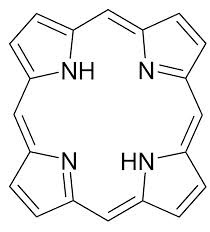
\includegraphics[scale=0.5]{graphics/porphin}
\caption{Porphin: Grundstruktur von Porphyrinen}
\end{figure}
Natürliche Porphyrine sind durch ihre Substituenten charakterisiert. Bei der Biosynthese entstehen zunächst die Porphyrinogenderivate, die einen höheren Sättigungsgrad besitzen und durch Dehydrierung zu Porphinderivaten werden. Eine für ihre biologische Funktion wichtige Eigenschaft ist ihre Neigung zur Chelatbildung von Metallen (Fe, Mg, Zn). Viele Eisen-Porphyrinverbindungen zeigen eine tiefrote Farbe.\cite{[8]}
\begin{figure}
\centering
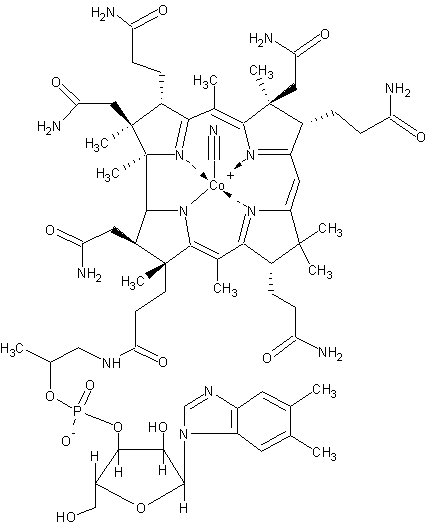
\includegraphics[scale=0.5]{graphics/Vitamin_B12}
\caption{Vitamin B 12}
\end{figure}
\begin{figure}[!htpb]
\centering
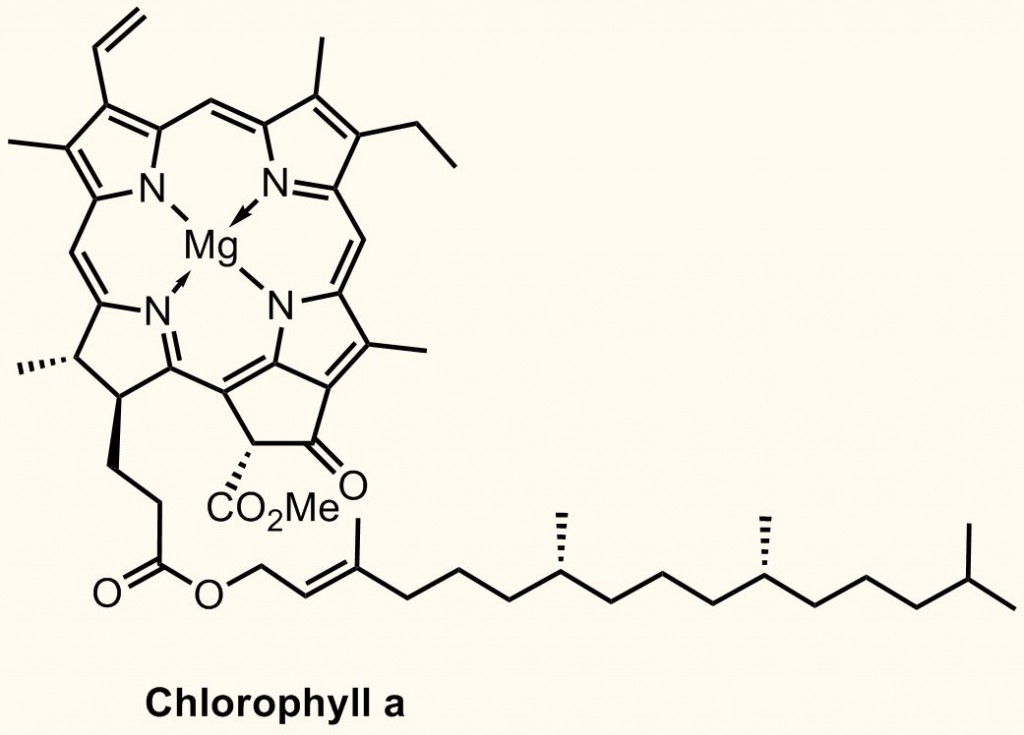
\includegraphics[scale=0.5]{graphics/Chlorophylla}
\caption{Chlorophyll A}
\end{figure}

\begin{figure}[!htpb]
\centering
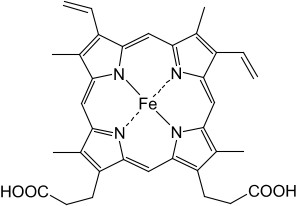
\includegraphics[scale=0.5]{graphics/haem3}
\end{figure}

\section{Arylethinylporphyrine}
\begin{figure}[!htpb]
\centering
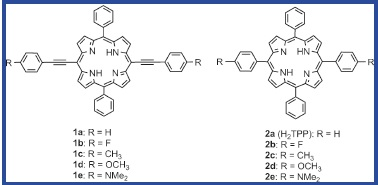
\includegraphics[scale=1]{graphics/arylethinylporphyrin}
\caption{Arylethinylporphyrine}
\end{figure}
Die Ethninyl-Funktionalität verlängern das konjugierte $\pi$-System des Porphyrins und entfernt die sterische Barriere zwischen Phenylgruppe und dem Porphyrin-Makrozyklus und erweitert die Konjugation über die Achsen des Moleküls. Solche Modifikationen führen zu Rotverschiebungen der B- und Q-Regionen. Die erweiterte Konjugation erleichtert die elektronische Kommunikation zwischen Porphyrin und den funktionellen Gruppen.
\\Arylethinyl Porphyrine werden in verschiedenen Bereichen, z.B. künstliche photosynthetische Systeme oder nichtlineare optische Materialien angewendet. Während Metall (Zn, Cu, Ni, Fe) Arylethinylporphyrine weit erforscht sind, gibt es nur wenige Studien zu metallfreien Arylethinylporphyrinen. Unter den richtigen Bedingungen, weisen manche metallfreie Porphyrine Hyperporphyrin-Spektren auf, die nicht mit den Vier-Orbital-Porphyrin-Model beschrieben werden können. Stattdessen entsteht ein Charge-Transfer-Übergang zwischen Substituent und Porphyrin-Ring. Diese Übergänge entstehen bei niedrigerer Energie und mit höherer Intensität als normale Porphyrin Q-Band Übergänge. 
\\Protonierung an den zentralen Stickstoff-Atomen resultiert in nichtplanare Verzerrungen im Porphyrin-Makrozyklus und bewirkt eine Veränderung in den photophysikalischen Eigenschaften wie rotverschobene Absorptions-Spektren, größeren Stokes-Shift, größere Fluoreszenzlinien und verkürzte Anregungs-Lebensspanne. \cite{[9]}
\section{$\pi$-erweiterte Porphyrine}
Porphyrine, die über Verschmelzung mit externen aromatischen Ringen erweitert wurden, besitzen rot-verschobene Absorptionsbanden und starke Lumineszenz bei Raumtemperatur. Die einfachsten Porphyrine in dieser Gruppe, meso-tetraaryltetrabenzoporphyrine wurden schon in biomedizinischen und nichtlinearen optischen Anwendungen benutzt. Tetranaphtoporphyrine wurden nur wenig studiert. Die Erweiterung auf Naphtalo am Pyrrolring führt zu einer Reihe von isomerischen Tetranaphthaloporphyrinen. Tetra[2,3]naphthaloporphyrine (TNP) und meso-tetraaryltetra[2,3]-naphthaloporphyrine (Ar$_4$TNP) sind höher symmetrisch und haben stärkere spektrale Übergänge.
\begin{figure}[!htbp]
\centering
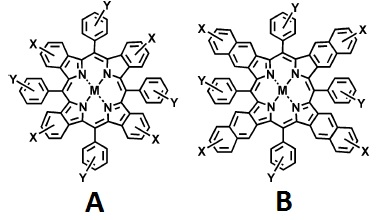
\includegraphics[scale=1]{graphics/MAr4TBP}
\caption{(A) tetraaryltetrabenzoporphyrin und (B) tetranaphtotetrabenzoporphyrin}
\end{figure}
TNPs können durch die Retro-Diels-Alder Reaktion (Umkehrung der Diels-Alder-Reaktion, kann durch Energiezufuhr oder Säuren herbeigeführt werden) hergestellt werden. Diese Methode kann aber keine Substituenten in den aromatischen Ring einbinden.
\\Eine andere Methode wäre eine oxidative Aromatisierung vom Porphyrinen mit nichtaromatischen Cyclohexen-Ringen. Mit dieser Methode können polyfunktionialisierte Ar$_4$TBPs mit guten Ausbeuten synthetisiert werden, z.B. tetra[1,2]naphthaloporphyrine, mono[1,2] und di[1,2]naphtaloporphyrine und mono[2,3]naphthaloporphyrine. \cite{[10]}
\begin{figure}[!htbp]
\centering
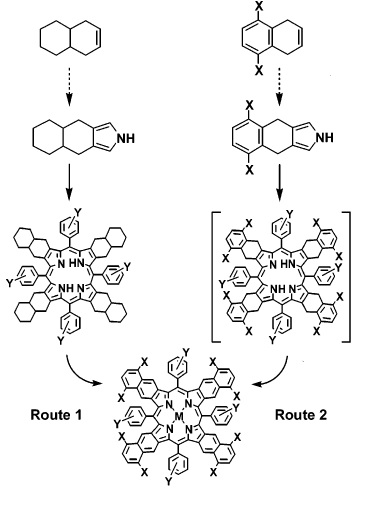
\includegraphics[scale=0.5]{graphics/oxidative_Aromatisierung}
\caption{oxidative Aromatisierung}
\end{figure}
Eine dritte Methode wäre die Template-Synthese
\subsection{meso-meso verknüpfte Porphyrine}
\begin{figure}[!htbp]
\centering
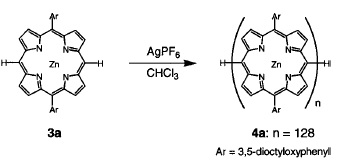
\includegraphics[scale=1]{graphics/meso-meso-fused}
\caption{Synthese von meso-meso-verknüpften Porphyrinen}
\end{figure}
Meso-meso-konjugierte Porphyrine wurden mittels Ag-unterstützten meso-meso-Kuppeln von 5,15-diaryl-substituierten Zn(II)-Porphyrinen zu bis zu 128-teiligen Porphyrinen verknüpft. Diese sollte eines der längsten von Menschen hergestellten Molekülen überhaupt sein. Dieses 128mer ist in organischer Lösemittel löslich. Mittels Gel-Permeations-Chromatographie konnten diese sehr langen Moleküle getrennt werden.
\cite{[11]}
\subsection{direkt verknüpfte Diporphyrine}
\begin{figure}[htpb]
\centering
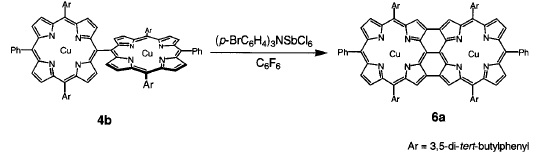
\includegraphics[scale=1]{graphics/diporphyrins}
\caption{Synthese von direkt-verknüpften Diporphyrinen}
\end{figure}
Zwei Porphyrin Ringe können verknüpft werden um eine coplanare Strukur zu bilden. Diese zeigen eine gepackte orthogonale Kristallstruktur, bei der die 3,5-di-tert-butylphenyl-Gruppe zum Cu(II)-diporphyrin zeigt. Es wird so zu einem unendlichen Netzwerk mit mehrern CH/$\pi$ -Wechselwirkungen.
\\Für 6a erkennt man ein Q-Band bei 994 nm (nach rot-verschoben).\cite{[11]}


